\documentclass[a4paper,11pt]{article}
\usepackage[utf8]{inputenc}
\usepackage[T1]{fontenc}
\usepackage{graphicx}
\usepackage{amsmath}
\usepackage{geometry}
\usepackage{amssymb}
\geometry{margin=2.5cm}

\title{Documentazione della Pipeline Immagini \\ \texttt{xai\_img}}

\begin{document}
\maketitle

\section*{1. Contesto}
è stata implementata una pipeline per analizzare il \emph{Disagreement Problem} su spiegazioni visuali: si confrontano due mappe di salienza generate dallo stesso modello (o da modelli diversi) su una medesima immagine, quantificando la loro divergenza con quattro metriche.

\section*{2. Tecnologie e librerie}
È stato utilizzato Python 3.10 in ambiente \texttt{conda (xai)}, con:
\begin{itemize}
  \item \textbf{PyTorch} e \textbf{torchvision} per il caricamento di una rete pre‐addestrata (ResNet-18);
  \item \textbf{Captum} per i metodi di interpretazione Integrated Gradients e Saliency;
  \item \textbf{scikit-image} per il caricamento e la segmentazione SLIC in super‐pixel;
  \item \textbf{NumPy} per la manipolazione delle mappe di salienza;
  \item \textbf{Matplotlib} per la visualizzazione finale delle heat‐map.
\end{itemize}

\section*{3. Metodi di interpretazione}
\subsection*{3.1 Integrated Gradients (IG)}
Integrated Gradients è un explainer che stima l’importanza di ciascun pixel (o feature) calcolando l’integrale del gradiente lungo un percorso che va da un \emph{baseline} (un’immagine nera) all’input reale.  
In pratica:
\begin{enumerate}
  \item si definisce un \emph{baseline} $x'\,$ (vettore di zeri);
  \item si suddivide il segmento $[x',x]$ in $m$ passi e si calcolano i gradienti in punti intermedi;
  \item si sommano i gradienti e si moltiplica per la variazione $x - x'$ per ottenere un valore di attributo per ciascun pixel.
\end{enumerate}
Aumentando $m$ (\texttt{n\_steps}) l’approssimazione diventa più fedele all’integrale continuo ma aumenta il costo computazionale. (se non viene passato \texttt{n\_steps}, Captum userà \texttt{n\_steps = 50} di default)

\subsection*{3.2 Saliency (gradiente puro)}
Il metodo \emph{Saliency} è la forma più semplice di explainability basata sul gradiente: 
si calcola il gradiente dell’output di interesse rispetto all’input, pixel per pixel.  
Il valore assoluto di questo gradiente indica quanto la predizione cambierebbe modificando lievemente quel pixel.  
Rispetto a IG, Saliency:
\begin{itemize}
  \item è istantaneo (un solo backward pass);
  \item tende ad essere più “rumoroso”;
  \item non richiede un \emph{baseline} né parametri aggiuntivi.
\end{itemize}

\section*{4. Flusso di lavoro}
La pipeline si articola in due fasi: generazione delle mappe di salienza e confronto quantitativo e visivo.

\subsection*{4.1 Generazione delle mappe (\texttt{make\_maps.py})}
\begin{enumerate}
  \item Caricamento di ResNet-18 con pesi ImageNet: 
    \texttt{models.resnet18(weights=ResNet18\_Weights.DEFAULT)}.
  \item Preprocessing dell’immagine (\texttt{cat.jpg}): resize a 224×224, conversione in tensore, normalizzazione.
  \item Predizione della classe di riferimento: 
    \texttt{pred = model(x).argmax()}.
  \item Baseline: vettore di zeri di forma $(1,3,224,224)$ per IG.
  \item Calcolo di:
    \begin{itemize}
      \item \texttt{IntegratedGradients.attribute(x, baselines=x*0, target=pred)} → mappa IG
      \item \texttt{Saliency.attribute(x, target=pred)} → mappa gradiente puro
    \end{itemize}
  \item Salvataggio in \texttt{.npy}: \texttt{saliency\_A.npy}, \texttt{saliency\_B.npy}.
\end{enumerate}

\subsection*{4.2 Confronto delle mappe (\texttt{compare\_saliency.py})}
\paragraph{Ridimensionamento}
L’immagine originale viene riportata alle dimensioni delle mappe caricate.

\paragraph{Super‐pixel}
Si applica SLIC con $N_{\text{segments}}=200$ per aggregare pixel in blocchi omogenei, ottenendo $n_{\text{sp}}$ super‐pixel.

\paragraph{Vettori di salienza}
Per ogni super‐pixel si calcola la media della salienza:
\[
v_i = \frac{1}{|S_i|} \sum_{(x,y)\in S_i} \text{saliency}(x,y),
\]
da cui si ottengono due vettori $\mathbf v^{(A)}, \mathbf v^{(B)}\in\mathbb R^{n_{\text{sp}}}$.

\paragraph{Metriche di disaccordo}
Si applicano:
\begin{itemize}
  \item \emph{Feature Disagreement}: $1 - \frac{|\mathrm{Top}_k(\mathbf v^{(A)})\cap\mathrm{Top}_k(\mathbf v^{(B)})|}{k}$;
  \item \emph{Sign Disagreement}: penalizza differenze di segno;
  \item \emph{Euclidean}: distanza $L_2$ tra vettori normalizzati;
  \item \emph{Euclidean‐abs}: distanza $L_2$ tra moduli normalizzati.
\end{itemize}
Impostata $K_{\text{FRAC}}=0.05 \implies k=0.05\,n_{\text{sp}}$.

\section*{5. Risultati}
Eseguendo:
\begin{verbatim}
python make_maps.py
python compare_saliency.py
\end{verbatim}
si ottiene:
\[
\begin{aligned}
\text{FeatureDisagreement} &= 1.000,\\ 
\text{SignDisagreement}    &= 1.000,\\
\text{Euclidean}           &= 1.417,\\
\text{Euclidean-abs}       &= 0.856.
\end{aligned}
\]
Questi valori indicano disaccordo massimo sulle top‐5\% di super‐pixel e grande distanza globale, confermando che le due mappe (IG vs Saliency) evidenziano aree significativamente diverse.

\subsection*{5.1 Interpretazione quantitativa}
\begin{itemize}
\item \textbf{FeatureDisagreement = 1.000}: fra i super‐pixel “top‐k” scelti da saliency A e quelli scelti da saliency B, non c’è alcuna sovrapposizione (100\% di disaccordo).
\item \textbf{SignDisagreement = 1.000}: anche considerando il segno dell’attribuzione (positivo vs negativo), non c’è alcuna corrispondenza nelle stesse regioni.
\item \textbf{Euclidean $\approx$ 1.417}: misura “globale” di distanza $L_2$ fra le due distribuzioni di saliency (vettori normalizzati): quindi le due mappe sono molto diverse.
\item \textbf{Euclidean‐abs $\approx$ 0.856}: stessa distanza ma ignorando il segno: resta elevata, il che conferma che anche le intensità “in assoluto” sono molto differenti.
\end{itemize}

\section*{6. Le tre immagini}
\begin{figure}[htbp]
\centering
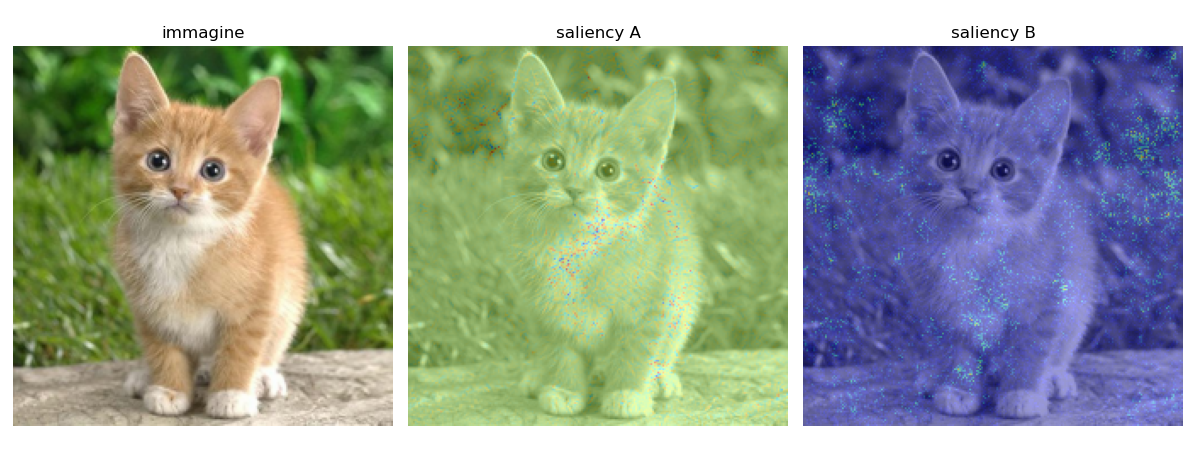
\includegraphics[height=3.5cm]{saliency.png}\qquad
\caption{Da sinistra: immagine originale, heat‐map IG (saliency A), heat‐map Saliency (saliency B).}
\label{fig:three_images}
\end{figure}

\subsection*{6.1 Immagine originale}
La foto originale (\texttt{cat.jpg}), ridimensionata a 224×224 pixel per coincidere con le mappe.

\subsection*{6.2 Saliency A}
Overlay della mappa generata con Integrated Gradients. I colori (scala dal verde al rosso, mappati con \texttt{plt.cm.jet}) mostrano le aree che IG ritiene importanti: più una zona è “rossastra”, più pesa sulla decisione del modello. Qui emerge una colorazione diffusa, con pochissime aree calde concentrate.

\subsection*{6.3 Saliency B}
Overlay della mappa generata con il metodo Saliency (gradiente puro). Qui il colore prevalente è bluastro, con pochi puntini verde‐chiaro che indicano dove il gradiente è massimo.

\section*{7. Discussione sul Disagreement Problem}
Nessuna sovrapposizione nelle aree top‐k (FeatureDisagreement = 1) → IG e gradiente puro indicano regioni completamente diverse come “più importanti”.

Anche le intensità complessive non sono vicine (Euclidean = 1.417) → l’intero pattern di saliency è distante.

Visivamente, IG ha evidenziato una zona ampia e sfumata (al centro del manto), mentre Saliency ha punti sparsi in tutta l’immagine.

Due explainers, applicati allo stesso modello e alla stessa immagine, raccontano storie molto diverse su quali pixel abbiano spinto la predizione.

\end{document}
